\documentclass[12pt]{article}
\usepackage[utf8]{inputenc}
\usepackage{lineno}
\usepackage{authblk}
\usepackage[margin=1in]{geometry}
\usepackage{xparse}
\usepackage{xpunctuate}
\usepackage{xspace}
\usepackage{graphicx}
\usepackage{wrapfig}
\usepackage[hidelinks]{hyperref}
\usepackage[all]{hypcap}
\usepackage{amsmath}
\usepackage{cleveref}
\usepackage{placeins}
\usepackage{flafter}
\usepackage{floatrow}
\usepackage{minted} 
\usepackage{caption}
\usepackage{float}
\usepackage{csvsimple}
\usepackage{booktabs}
\usepackage{siunitx}

% local definitions
\newcommand{\msprime}[0]{\texttt{msprime}\xspace}
\newcommand{\tskit}[0]{\texttt{tskit}\xspace}
\newcommand{\slim}[0]{\texttt{SLiM}\xspace}
\newcommand{\pyslim}[0]{\texttt{pyslim}\xspace}
\newcommand{\allel}[0]{\texttt{scikit-allel}\xspace}
\newcommand*{\eg}{e.g.\xcomma}
\newcommand*{\ie}{i.e.\xcomma}
\newcommand{\comment}[1]{\textit{\color{green} #1}}

% syntax highlighting
\usepackage{listings}
\usepackage{xcolor}

% see listings documentation
\lstdefinelanguage{slim}{
    % Eidos language keywords from 
    % https://github.com/MesserLab/SLiM/blob/4bcc36a02aeacdc9ee808e38d62836f854246502/eidos/eidos_token.h#L90
    morekeywords=[1]{if,else,do,while,for,in,next,break,return,function},
    % SLiM callback keywords from
    % https://github.com/MesserLab/SLiM/blob/4bcc36a02aeacdc9ee808e38d62836f854246502/core/slim_eidos_block.cpp#L32
    morekeywords=[2]{first,early,late,initialize,mutationEffect,fitnessEffect,interaction,mateChoice,modifyChild,recombination,mutation,survival,reproduction},
    % Other special SLiM tokens from
    % https://github.com/MesserLab/SLiM/blob/4bcc36a02aeacdc9ee808e38d62836f854246502/QtSLiM/QtSLiMSyntaxHighlighting.cpp#L294
    morekeywords=[3]{sim,community,slimgui,
        p0,p1,p2,p3,p4,p5,p6,p7,p8,p9,p10,p11,p12,p13,p14,p15,p16,p17,p18,p19,p20,p21,p22,p23,p24,p25,
        p26,p27,p28,p29,p30,p31,p32,p33,p34,p35,p36,p37,p38,p39,p40,p41,p42,p43,p44,p45,p46,p47,p48,p49,p50,
        g0,g1,g2,g3,g4,g5,g6,g7,g8,g9,g10,g11,g12,g13,g14,g15,g16,g17,g18,g19,g20,g21,g22,g23,g24,g25,
        g26,g27,g28,g29,g30,g31,g32,g33,g34,g35,g36,g37,g38,g39,g40,g41,g42,g43,g44,g45,g46,g47,g48,g49,g50,
        m0,m1,m2,m3,m4,m5,m6,m7,m8,m9,m10,m11,m12,m13,m14,m15,m16,m17,m18,m19,m20,m21,m22,m23,m24,m25,
        m26,m27,m28,m29,m30,m31,m32,m33,m34,m35,m36,m37,m38,m39,m40,m41,m42,m43,m44,m45,m46,m47,m48,m49,m50,
        s0,s1,s2,s3,s4,s5,s6,s7,s8,s9,s10,s11,s12,s13,s14,s15,s16,s17,s18,s19,s20,s21,s22,s23,s24,s25,
        s26,s27,s28,s29,s30,s31,s32,s33,s34,s35,s36,s37,s38,s39,s40,s41,s42,s43,s44,s45,s46,s47,s48,s49,s50,
        i0,i1,i2,i3,i4,i5,i6,i7,i8,i9,i10,i11,i12,i13,i14,i15,i16,i17,i18,i19,i20,i21,i22,i23,i24,i25,
        i26,i27,i28,i29,i30,i31,i32,i33,i34,i35,i36,i37,i38,i39,i40,i41,i42,i43,i44,i45,i46,i47,i48,i49,i50},
    sensitive=true,
    morecomment=[l]{//},
    morestring=[b]",
}
% colors from 
% https://github.com/MesserLab/SLiM/blob/4bcc36a02aeacdc9ee808e38d62836f854246502/QtSLiM/QtSLiMSyntaxHighlighting.cpp#L139
% numberLiteralFormat.setForeground(inDarkMode ? QColor(115, 145, 255) : QColor(28, 0, 207));
% stringLiteralFormat.setForeground(inDarkMode ? QColor(220, 98, 90) : QColor(196, 26, 22));
% commentFormat.setForeground(inDarkMode ? QColor(90, 210, 90) : QColor(0, 116, 0));
% identifierFormat.setForeground(inDarkMode ? QColor(70, 205, 216) : QColor(63, 110, 116));
% keywordFormat.setForeground(inDarkMode ? QColor(220, 83, 185) : QColor(170, 13, 145));
\definecolor{slimstring}{RGB}{196,26,22}
\definecolor{slimcomment}{RGB}{0,116,0}
\definecolor{slimidentifier}{RGB}{63,110,116}
\definecolor{slimkeyword}{RGB}{170,13,145}
\definecolor{slimstage}{RGB}{0,0,0}
\definecolor{codegray}{RGB}{128,128,128}
% Light beige background for SLiM code (different from Python's gray background)
\definecolor{backcolour}{rgb}{0.95,0.95,0.92}
\lstdefinestyle{slimstyle}{
    language=slim,
    backgroundcolor=\color{backcolour},
    commentstyle=\color{slimcomment},
    keywordstyle=[1]\color{slimkeyword},
    keywordstyle=[2]\color{slimstage},
    keywordstyle=[3]\color{slimidentifier},
    numberstyle=\tiny\color{codegray},
    stringstyle=\color{slimstring},
    basicstyle=\ttfamily\small,
    escapeinside={*@}{@*},
    breakatwhitespace=false,         
    breaklines=true,                 
    captionpos=b,                    
    keepspaces=true,                 
    numbers=left,                    
    numbersep=2pt,                  
    showspaces=false,                
    showstringspaces=false,
    showtabs=false,                  
    tabsize=2
}
\lstset{style=slimstyle}

% Fix for quote encoding issues
% https://tex.stackexchange.com/questions/736299/latex-error-command-textquotedbl-unavailable-in-encoding-ot1
\lstset{upquote=true,basicstyle=\fontencoding{T1}\selectfont}

\definecolor{bg}{rgb}{0.95,0.95,0.98}
\newminted[pycon]{pycon}{bgcolor=bg, linenos=true, tabsize=4}

%\linenumbers

\begin{document}

\title{Bridging forward-in-time and coalescent simulations using pyslim}
\author[1]{Shyamalika Gopalan}
\author[2,3]{Murillo F. Rodrigues}
\author[3,4]{Peter L. Ralph}
%\author[5]{Ben Haller}

\affil[1]{Department of Genetics and Biochemistry and Center for Human Genetics, Clemson University}
\affil[2]{Division of Genetics, Oregon National Primate Center, Oregon Health \& Science University}
\affil[3]{Department of Biology and Institute of Ecology and Evolution, University of Oregon}
\affil[4]{Department of Mathematics, University of Oregon}
%\affil[5]{Department of Computational Biology, Cornell University}

\maketitle

\abstract{
Lorem ipsum
}
\date{}

\section*{Introduction}
% The importance of simulations in popgen and flavors of simulations
Simulations have been an invaluable tool in population genetics for the past six decades.
%because of the difficulty in obtaining analytical solutions to complex evolutionary scenarios.
The two main strategies for population genetic simulation differ in the direction of the process: forward or backward-in-time.
The coalescent process models the ancestry of sampled genomes back in time until they coalesce into one most common recent ancestor (MRCA).
It is perhaps the most common framework for population genetic simulation because of its efficiency:
it bypasses the need to represent entire populations in memory and the sampling of gametes every generation.
Despite its efficiency, the coalescent has strict assumptions (\eg neutrality) which limits applicability.
Forward-in-time simulations starts with actual individuals and applies evolutionary rules (\eg mutation, recombination, selection) over generations until a certain criterion is met.
Thus, forward-in-time simulations are much more flexible, but they come with a high computational cost.

% The tree sequence and its utility in bridging forward-in-time and coalescent simulations
Recent advancements both in computational power and software development have made simulations much more accessible and popular.
A key development that has decreased the computational cost of simulations is the tree sequence,
a data structure that concisely encodes correlated genealogies along the genome.
In the context of forward-in-time simulations,
the recording of tree sequences increases efficiency because it allows for
(i) the omission of neutral mutations during the simulation process, and
(ii) the use of fast coalescent as a neutral "burn-in" phase,
such that the forward simulation can begin with an equilibrium level of genetic diversity.
Further, using tree sequences it is possible to bridge forward and backwards methods, 
for example by using the coalescent to ensure all lineages coalesce into a single common ancestor (a process called \"recapitation\").

% The pyslim package and overview of the chapter
Here, we present \pyslim, a Python package for reading and modifying \tskit tree sequences produced by
the popular coalescent and forward-in-time simulation tools such as \slim and \msprime.
\pyslim provides a way to perform \"hybrid\" simulations, combining both forwards and backwards (coalescent) methods.
We will describe the main uses of \pyslim: (i) recapitation, which is the process of filling in the history of the first-generation individuals which have not coalesced, (ii) generation of initial diversity for forward-in-time simulations, (iii) parallelization of multi-species simulations, and (iv) complex simulation of alternating life cycles.

\section*{Starting with diversity generated by coalescent simulation}

Simulations of large populations with selection can be costly,
especially because we might need to run a lengthy “burn-in” period to get the genetic variation for selection to act on.
Because the precise form of the burn-in may not be important, 
a neutral burn-in can be efficiently run with coalescent simulator such as \msprime.
In this section, we will demonstrate how to perform such a hybrid simulation using \pyslim, \msprime and \slim.

Imagine the scenario where we perform a lab experiment in which
we take high-diversity organisms from the wild and subject them to selection for a few dozen generations.
Although genetic diversity in the wild is most likely not neutral,
we do not know precisely what it does look like and a coalescent simulation would be an acceptable starting point.
The key attribute of reality we would like to approximate is the joint distribution of allele frequencies and effect sizes.
If the alleles affect a trait under stabilizing selection,
we would expect a negative correlation between the two.
On the other hand, there would be no relationship between allele frequencies and effect sizes
if the trait we are selecting on in the lab is not under strong selection in the wild.
We will simulate the scenario where the trait we put under selection in the lab is not under stabilizing selection in the wild.
To do so, we will:

\begin{enumerate}
    \item Run a coalescent simulation with msprime.

    \item Add \slim metadata to the nodes, individuals, and populations.

    \item Add \slim mutations with msprime, and edit the mutation metadata to assign selection coefficients.

    \item Run the \slim portion of the simulation.

    \item Do some descriptive analysis of the results of selection.

    \item Add neutral mutations to the tree sequence.

    \item Do some descriptive analysis of genetic diversity along the genome.
\end{enumerate}

\subsection*{Variable mutation rate map}

In this model, we will also demonstrate how to modulate the mutation rate along the genome.
We will partition the 9Mbp genome in three equally-sized domains.
The total mutation rate along the genome will be constant (\num{3e-8} per generation per bp).
In the first and last third of the genome, 1\% of mutations are beneficial with a selection coefficient drawn from an Exponential distribution.
In the middle third, only 0.1\% of mutations are beneficial (but with the same distribution of selection coefficients).
This implies that the mutation rate of beneficial mutations on the ends is \num{3e-10} per generation per bp, and in the middle is \num{3e-11} per generation per bp.
First, we will simulate the beneficial mutations under these different mutation rates.
Then, to ensure the total mutation rate along the genome is constant, we will add neutral mutations at rates \num{2.97e-8} the ends, and \num{2.997e-8} in the middle.


 \subsection*{The coalescent simulation}

 First, we will use \msprime to simulate the evolutionary history of 1,000 diploid samples from a population of size 50,000.

\comment{(commented-out code block that wasn't compiling)}
%  \begin{listing}[H]
%   \begin{minted}[fontsize=\small, linenos, bgcolor=gray!10]{python}
% demog_model = msprime.Demography()
% demog_model.add_population(initial_size=50_000)
% ots = msprime.sim_ancestry(
%     samples=1_000,
%     demography=demog_model,
%     random_seed=5,
%     recombination_rate=1e-8,
%     sequence_length = 9_000_000)
%   \end{minted}
% \end{listing}

\subsection*{Annotating tree sequence with SLiM metadata}

At this point, we have genealogical information: individuals, nodes (chromosomes), and relationships between them,
but no genetic diversity; no mutations. 
First, we will add SLiM metadata to all of these things, a procedure we call “annotating”.
\begin{listing}[H]
  \begin{minted}[fontsize=\small, linenos, bgcolor=gray!10]{python}
ots = pyslim.annotate(ots, model_type="WF", tick=1, stage="late")
  \end{minted}
\end{listing}

This \pyslim method adds default metadata to everything that needs it:
in this case, all individuals, all nodes that are part of alive individuals, and all populations referenced by nodes.
These default values are returned by \verb|slim_default_metadata()| (e.g., all individuals are hermaphrodite, all chromosomes are autosomal).

\subsection*{Adding mutations with SLiM metadata}

Next, we will use the \verb|msprime.SLiMMutationModel| to add mutations to the tree sequence.
These will carry SLiM metadata, but this metadata will say that the mutations are neutral.
So, we will later need to modify their metadata after the fact to have selection coefficients drawn from some distribution.
Remember, our motivation here is that we are using \msprime to obtain a plausible level of functional standing genetic variation on which selection can act:
imagine that the mutations were (nearly) neutral in the wild, but then became subject to strong selection in the lab, for some reason.
We will want this to be as if we'd done it in a burn-in script in \slim :

\begin{lstlisting}{language=slim}
    initialize() {
        ...
        initializeMutationType("m2", 0.5, "e", 0.04);
        initializeMutationRate(3e-10);
     }
  
     fitness(m2) {
         return 1.0;
     }
\end{lstlisting}

In other words, we would like to pull selection coefficients from an exponential distribution with mean 0.04
(but, of course, this is a coalescent simulation, so the dynamics of the mutations up until this point have been neutral).
Note that the dominance coefficient is not stored in the tree sequence:
it gets set in the SLiM recipe because it is a property of the mutation type, not of individual mutations, in SLiM.
Here is how to add SLiM mutations with \msprime :

\begin{listing}[H]
    \begin{minted}[fontsize=\small, linenos, bgcolor=gray!10]{python}
mut_map = msprime.RateMap(
           position=breaks,
           rate=[0.03e-8, 0.003e-8, 0.03e-8])
mut_model = msprime.SLiMMutationModel(type=2)
ots = msprime.sim_mutations(
            ots,
            rate=mut_map,
            model=mut_model,
            keep=True, 
            random_seed=12)
print(f"The tree sequence now has {ots.num_mutations} mutations, at "
          f"{ots.num_sites} distinct sites.")
  \end{minted}
\end{listing}

\begin{pycon}
The tree sequence now has 309 mutations, at 309 distinct sites.
\end{pycon}

Note the type=2 argument to \verb|msprime.SLiMMutationModel|:
this means the mutations will be of type “m2” in SLiM
(and, so you must initialize that mutation type in the recipe that loads this tree sequence in).

Now, we will assign selection coefficients.
Recall that to accomodate mutation stacking in SLiM,
a mutation metadata entry is in fact a list of metadata entries,
one for each of the SLiM mutations that are stacked at this position.
The SLiM IDs of these mutations are available (in the same order) as a comma-separated list of integers in the derived state of the mutation.
So, in case some SLiM mutations appear in more than one mutation in the tree sequence,
we will build a map from SLiM ID to selection coefficient:
\verb|mut_map[k]| will give the selection coefficient of the SLiM mutation with SLiM mutation ID \verb|k|.

\begin{listing}[H]
    \begin{minted}[fontsize=\small, linenos, bgcolor=gray!10]{python}
rng = np.random.default_rng(seed=1234)
tables = ots.tables
tables.mutations.clear()
mut_map = {}
for m in ots.mutations():
  md_list = m.metadata["mutation_list"]
  slim_ids = m.derived_state.split(",")
  assert len(slim_ids) == len(md_list)
  for sid, md in zip(slim_ids, md_list):
     if sid not in mut_map:
        mut_map[sid] = rng.exponential(scale=0.04)
     md["selection_coeff"] = mut_map[sid]
  _ = tables.mutations.append(
          m.replace(metadata={"mutation_list": md_list})
  )

# check we didn't mess anything up
assert tables.mutations.num_rows == ots.num_mutations
print(f"The selection coefficients range from {min(mut_map.values()):0.2e}")
print(f"to {max(mut_map.values()):0.2e}.")
  \end{minted}
\end{listing}
\begin{pycon}
The selection coefficients range from 1.13e-10 to 3.70e-01.
\end{pycon}

\subsection*{Loading into SLiM}
Before loading the tree sequence into SLiM,
we should check the top-level metadata.
We can see this with \verb|tables.metadata|:

\begin{listing}[H]
    \begin{minted}[fontsize=\small, linenos, bgcolor=gray!10]{python}
tables.metadata
    \end{minted}
\end{listing}
\begin{pycon}
{
    'SLiM': {
        'cycle': 1, 
        'description': '', 
        'file_version': '0.8', 
        'model_type': 'WF', 
        'name': '', 
        'nucleotide_based': False, 
        'separate_sexes': False, 
        'spatial_dimensionality': '', 
        'spatial_periodicity': '', 
        'stage': 'late', 
        'tick': 1
        }
}
\end{pycon}

We should edit this to match our planned slimulation particularly the \verb|model_type| (WF or nonWF) and the \verb|tick|.
The \verb|tick| tells SLiM what value to set the tick counter to once this tree sequence is loaded.
In principle, it can be set to anything, independently of the times in the tree sequence,
because the times in the tree sequence are measured in units of “time before the end”;
and the tick that gets passed to SLiM sets what that “end time” is, in SLiM’s time.
However, if you change this, the \verb|slim_time| attributes in mutation metadata will not be accurate.
This is harmless, unless you do something with mutations’ times yourself.

The model type is already Wright-Fisher,
but just to demonstrate how to edit the metadata,
and then we’ll write the tree sequence to a file.

\begin{listing}[H]
    \begin{minted}[fontsize=\small, linenos, bgcolor=gray!10]{python}
ts_metadata["SLiM"]["model_type"] = "WF"
tables.metadata = ts_metadata
ots = tables.tree_sequence()
ots.dump("vignette_annotated.init.trees")
    \end{minted}
\end{listing}   

Now, we can move onto the SLiM recipe.
This simply continues selected mutations as before (with mutation rate \num{1e-10} per bp per generation and the same distribution of fitness effects).
The population size is determined by the number of individuals that were read in from the tree sequence.
We need to make sure that the genome lengths match, so we provide that as a constant \verb|L|, that will be provided at run time.
To facilitate later analysis, we’ll also “Remember” the individuals present at the start of the simulation,
so that they will remain in the tree sequence.

\comment{(attempt to input a ipynb here)}
% \begin{listing}[H]
%     \inputminted[fontsize=\small, linenos, bgcolor=gray!10]{python}{./code/generating_diversity/generating.ipynb}
% \end{listing}

Note that the simulation only has selected mutations (of type \verb|m2|),
but as we will add in type \verb|m1| mutations later,
we have declared them in the recipe as a placeholder.

We could run this on the command line as \verb|slim -d L=100000000 reload_annotated.slim|,
but this time we will stay within python, and obtain the sequence length programatically:

\begin{pycon}
    // Initial random seed:
    5
    
    // RunInitializeCallbacks():
    initializeSLiMModelType(modelType = 'WF');
    initializeTreeSeq();
    initializeMutationRate(c(3e-11, 3e-12, 3e-11), c(2999999, 5999999, 8999999));
    initializeMutationType(1, 0.5, "f", 0);
    initializeMutationType(2, 0.5, "e", 0.1);
    initializeGenomicElementType(1, m2, 1);
    initializeGenomicElement(g1, 0, 8999998);
    initializeRecombinationRate(1e-08);
    
    // Starting run at tick <start>:
    1 
    
    Done.
\end{pycon}

\subsection*{Analyzing the resulting tree sequence}

First, let’s look at what mutations are present.

\comment{(commented-out code block that wasn't compiling)}
% \begin{listing}[H]
%     \begin{minted}[fontsize=\small, linenos, bgcolor=gray!10]{python}
% ts = tskit.load("vignette_annotated.trees")
% num_stacked = np.array([len(m.metadata["mutation_list"]) for m in ts.mutations()])
% init_time = ts.metadata['SLiM']['tick']
% old_mut = np.array([m.time > init_time - 1 - 1e-12 for m in ts.mutations()])
% assert sum(old_mut) == ots.num_mutations
% print(f"There are {ts.num_mutations} present at {ts.num_sites} distinct sites.")
% print(f"Of these, {np.sum(num_stacked > 1)} have more than one stacked mutation,")
% print(f"and {np.sum(old_mut)} were produced by msprime.")
%     \end{minted}
% \end{listing}
% \begin{pycon}
% There are 318 present at 318 distinct sites.
% Of these, 0 have more than one stacked mutation,
% and 309 were produced by msprime.
% \end{pycon}

Most of the mutations were present as initial diversity,
but a few were added during the course of the simulation.
Along the way we did a consistency check,
that the number of “old” mutations matches the number of mutations we had in the tree sequence we loaded into SLiM.
Since we ran SLiM for 500 time steps,
but loaded the tree sequence in during the \verb|late()| stage of time step 1,
the “old” mutations are those from at least 499 units of time ago
(and the \num{1e-12} is necessary for floating-point error).

A simple thing to look at next is:
how did the selected mutations change in frequency?
We can do this thanks to our having Remembered the first generation.
First, we will compute all allele frequencies among both the first generation and the final generation:

\begin{listing}[H]
    \begin{minted}[fontsize=\small, linenos, bgcolor=gray!10]{python}
times = list(set(ts.individuals_time))
times.sort()
print("The times ago at which individuals in the tree sequence were born:", times)
# The times ago at which individuals in the tree sequence were born: [0.0, 100.0]
nodes_by_time = [ts.samples(time=t) for t in times]

num_nodes = np.array([len(x) for x in nodes_by_time])
p = ts.sample_count_stat(nodes_by_time, lambda x: x/num_nodes, 2, windows='sites',
        strict=False, span_normalise=False, polarised=True)
s = np.array([sum([sum([md["selection_coeff"] for md in m.metadata["mutation_list"]])
                  for m in site.mutations]) for site in ts.sites()])
    \end{minted}
\end{listing}
\begin{pycon}
The times ago at which individuals in the tree sequence were born: [np.float64(0.0), np.float64(499.0)]
\end{pycon}

To do this, we used the \verb|time=t| argument to \verb|tskit.TreeSequence.samples()| to find the nodes alive at each of the two times (0 and 500 generations ago);
then computed an array \verb|p| of allele frequencies, with one row per site,
the first column giving the frequency among the initial generation,
and the second giving the frequency at the end.
We also pull out \verb|s|, the selection coefficients.
This last bit is complex because each site can have more than one mutation,
and each tree sequence mutation can represent more than one SLiM mutation.
And, the way we have dealt with this is a bit of a hack, so let’s look at that site with multiple mutations:

\begin{listing}[H]
    \begin{minted}[fontsize=\small, linenos, bgcolor=gray!10]{python}
for j, v in enumerate(ts.variants()):
  if len(v.site.mutations) > 1:
     print(f"Site {j} has {num_stacked[j]} stacked mutations, "
           f"with total derived allele frequency {p[j]} "
           f"and sum of selection coefficients {s[j]}.")
     print(f"The allele frequencies are:")
     for k, a in enumerate(v.alleles):
        print(f"  '{a}': {sum(v.genotypes == k)}")
     print(v.site)
    \end{minted}
\end{listing}

There were two mutations at this site, both before the SLiM portion of the simulation started.
One happened on the background of the other, and no genomes either today or in the initial generation carry the first allele in isolation.
Their effects combine in SLiM, so treating this as a single allele is correct.

Now, we will plot the initial and final allele frequencies, with point size and color determined by the selection coefficient:

\begin{listing}[H]
    \begin{minted}[fontsize=\small, linenos, bgcolor=gray!10]{python}
fig, ax1 = plt.subplots(figsize=(5, 4))
dp = ax1.scatter(p[:, 1], p[:,0], c=s, s=s*800, label='frequencies', norm=colors.LogNorm(vmin=s.min(), vmax=s.max()))
ax1.set_xlabel("initial allele frequency")
ax1.set_ylabel("final allele frequency")
fig.colorbar(dp, ax=ax1, label='selection coefficient');
    \end{minted}
\end{listing}

Unsurprisingly, mutations that had a large change in allele frequency seem to be biased towards ones with higher selection coefficients,
and those that were initially present at moderate frequency but were lost are biased towards smaller selection coefficients.

\subsection*{Overlaying neutral mutations}

In real data, of course, we do not get to observe selection coefficients.
We have not added in neutral mutations until this point for efficiency - they are just bookkeeping,
and do not affect the course of the simulation in any way.
For this reason, we can add them in after the fact,
in a way that is exactly equivalent to having kept track of them as we went along.

Recall that out of an overall mutation rate of 3e-8,
we wanted 99\% of the mutations to be neutral on the ends of the chromosome,
and 99.9\% to be neutral in the middle.
So, we will now add mutations at these rates, using the same model of mutation as before.
The code is nearly the same as before, with a few changes.
We have changed the type of the mutations (so that neutral mutations will show up in SLiM as \verb|m1|,
while selected mutations above were \verb|m2|),
and we have asked these mutations to have SLiM mutation IDs beginning at the ID where the previous mutations left off.
(This would be important were we to read this tree sequence back in to SLiM;
mutation IDs must be unique.)
And, importantly, we’ve added \verb|keep=True| so that existing mutations are not discarded.

\begin{listing}[H]
    \begin{minted}[fontsize=\small, linenos, bgcolor=gray!10]{python}
neutral_mut_map = msprime.RateMap(
           position=breaks,
           rate=[2.97e-8, 2.997e-8, 2.97e-8])
next_id = pyslim.next_slim_mutation_id(ts)
neutral_mut_model = msprime.SLiMMutationModel(
                                type=1,
                                next_id=next_id)
mts = msprime.sim_mutations(
                ts,
                rate=neutral_mut_map,
                model=neutral_mut_model,
                keep=True, 
                random_seed=35)
print(f"The tree sequence now has {mts.num_mutations} mutations,")
print(f"at {mts.num_sites} distinct sites.")
    \end{minted}
\end{listing}

\begin{pycon}
The tree sequence now has 443071 mutations, at 431899 distinct sites.
\end{pycon}

Now, we have a lot more mutations! And some of the sites have more than one mutation:

\begin{listing}[H]
    \begin{minted}[fontsize=\small, linenos, bgcolor=gray!10]{python}
num_alleles = np.array([len(s.mutations) for s in mts.sites()])
for k in range(1, max(num_alleles)+1):
  print(f"There are {sum(num_alleles == k)} sites with {k} distinct alleles.")
    \end{minted}
\end{listing}
\begin{pycon}
There are 420920 sites with 1 distinct alleles.
There are 10790 sites with 2 distinct alleles.
There are 185 sites with 3 distinct alleles.
There are 4 sites with 4 distinct alleles.
\end{pycon}

To get a nice a picture of what has happened, we will pull out a tree that had a lot of mutations on it,
and print a picture of it, with mutations labeled by their type:

\begin{listing}[H]
    \begin{minted}[fontsize=\small, linenos, bgcolor=gray!10]{python}
for t in mts.trees():
 mt = [max([u['mutation_type'] for u in m.metadata['mutation_list']]) for m in t.mutations()]
 if t.num_mutations > 12:
   break

ml = {m.id: str(mtype) for mtype, m in zip(mt, t.mutations())}
display(
    t.draw_svg(mutation_labels=ml,
               node_labels={},
               size=(400, 300))
)
    \end{minted}
\end{listing}

%TODO: add the FIG

On this tree each mutation is marked by a red “x”,
and labeled with its mutation type: either “1”, for newly added mutations, or “2”, for selected mutations present during the SLiM portion.
(Note: this is a large tree, with 68,211 nodes! But as usual, the main structure is visible because most nodes coalesce very recently.) % TODO: update numbers

OK, but how exactly is this working?
Can a neutral mutation be added to a site that previously had a selected mutation?
The short answer is: yes, and new alleles stack on top of existing alleles,
but existing alleles replace new alleles.
This is equivalent to including them as the simulation went along,
by the additivity property of Poisson mutations:
it turns out that the following two ways of generating mutations along the genome are equivalent:
either (\textit{a}) placing a random Poisson number with mean,
and randomly choosing each one to be non-neutral with probability 0.01, or
(\textit{b}) placing random, independent Poisson numbers of neutral and non-neutral mutations with means $0.99 \mu$ and $0.01 \mu$ respectively.
Since the neutral ones do not affect the simulation otherwise, we can add them in afterwards.
Now, when the mutation algorithm in \msprime puts down a new mutation at a site with mutations already existing,
it appends the newly generated SLiM mutation ID to the previous derived state,
and adds the metadata for the new SLiM mutation to the list of metadata from the previous mutation.
However, it does not modify any existing mutations, so their derived states (and metadata) are unchanged.
The result is that, from the point of view of SLiM, neutral (“m1”) mutations “stack” on top of any other mutations (neutral or selected), while selected (“m2”) mutations stack with each other, but replace any neutral mutations.
This “stacking policy” is not actually exactly implementable in SLiM,
but given that our newly added mutations are meant to be entirely neutral,
seems like a reasonable policy.
If you wanted some other arrangement (e.g., to have m1 stack on top of m2),
you could go through and modify derived states and metadata appropriately.

Let’s check there are any sites with stacked mutations of different types in the simulation. There is indeed one such site:

\begin{listing}[H]
    \begin{minted}[fontsize=\small, linenos, bgcolor=gray!10]{python}
for site in mts.sites():
  if len(site.mutations) > 1:
     types = [set([md["mutation_type"] for md in mut.metadata["mutation_list"]])
              for mut in site.mutations]
     if max(map(len, types)) > 1:
        print(site)
    \end{minted}
\end{listing}
\begin{pycon}
Site(id=427551, position=8911472.0, ancestral_state='', mutations=[Mutation(id=438595, site=427551, node=75771, derived_state='304', parent=-1, metadata={'mutation_list': [{'mutation_type': 2, 'selection_coeff': 0.017608141526579857, 'subpopulation': -1, 'slim_time': -82602, 'nucleotide': -1}]}, time=83102.9131115732, edge=469898), Mutation(id=438596, site=427551, node=9168, derived_state='304,438765', parent=438595, metadata={'mutation_list': [{'mutation_type': 2, 'selection_coeff': 0.017608141526579857, 'subpopulation': -1, 'slim_time': -82602, 'nucleotide': -1}, {'mutation_type': 1, 'selection_coeff': 0.0, 'subpopulation': -1, 'slim_time': -1041, 'nucleotide': -1}]}, time=1042.8889606594637, edge=104765)], metadata=b'')
\end{pycon}

%TODO edit this depending on output
Here, a neutral mutation has been put down on top of a selected mutation, but stacked,
so that any samples inheriting either of these mutations carries the selected mutation.
For more discussion of how this works, see  the documentation of \verb|msprime.SLiMMutationModel|.

\section*{What information is stored in the tree sequence}

A tree sequence is a way of storing both the full genetic history and the genotypes
of a bunch of genomes.
See CITE
for more description of the tree sequence and underlying data structure,
and definitions of the important terms.
Each (haploid) genome is associated with a \textit{node},
and the ``focal'' nodes are called \textit{sample nodes} or simply \textit{samples}.
Many operations on tree sequences act on the sample nodes by default,
and the tree sequence always describes the genealogy of the
entire genome of all the samples, at at least over the simulated time period.
(Other nodes in the tree sequence represent ancestral genomes
about which we might have only partial information).
SLiM simulates diploid organisms, so each \textit{individual} usually has two nodes;
many operations you might want to do involve first finding the individuals you want,
and then looking at their nodes.

\begin{figure}
\centering
    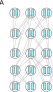
\includegraphics{figures/pedigree0}
    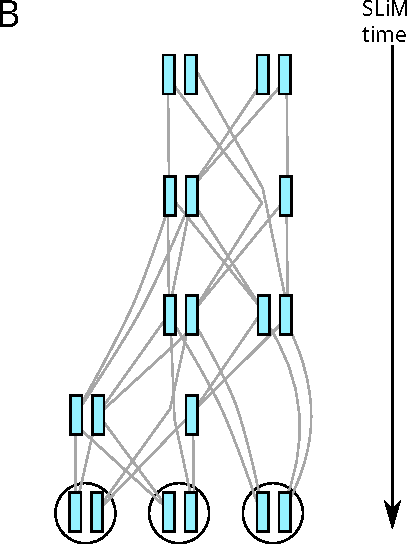
\includegraphics{figures/pedigree1}
    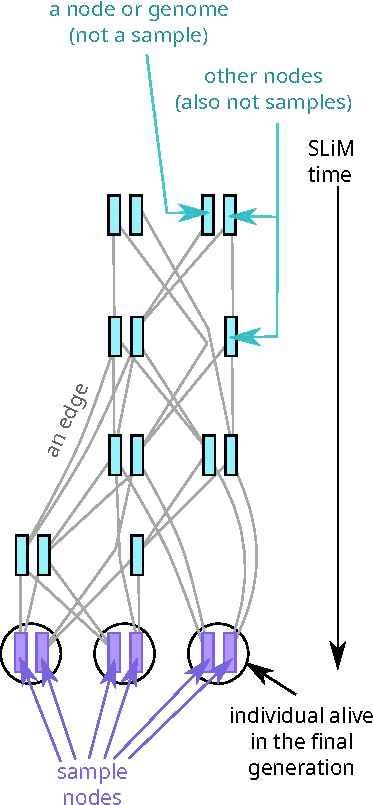
\includegraphics{figures/pedigree2}
\caption{
    \textbf{(A)} What happens in SLiM.
    \textbf{(B)} What we end up with at the end.
    \textbf{(C)} Labeled.
}
\label{fig:indivs}
\end{figure}



\paragraph{What does SLiM record in the tree sequence?}
Suppose we've run a very small simulation with SLiM. The genetic relationships between
the various diploid individuals who were alive over the course of the simulation might
look something like Figure~\ref{fig:indivs}A.
Note that individuals (circles) are
diploid, so that each contains two chromosomes or *nodes* (shaded rectangles),
and that relationships are between the *nodes*, not the individuals.

At the end of the simulation we are typically only interested in the genetic
relationships between the nodes in those individuals which are still alive;
other parts of the genealogy are irrelevant. To save having to store this unnecessary
genealogical information, SLiM *simplifies* the tree sequence as it goes along, retaining
only certain parts of the genetic genealogy. When the tree sequence is output, the result
then looks something like the situation in [the figure below](pedigree01), in which many of the nodes and
individuals have been removed.

\paragraph{Who and what is in the tree sequence?}

OK, who and what exactly *is* left in the tree sequence after the unnecessary
information has been removed?
Figure~\ref{fig:indivs}C depicts the terminology.
In the recorded tree sequence the individuals who are alive at the end of the simulation
have their nodes marked as \textit{samples},
and so we have their full genetic ancestry.
The sample nodes,
and the individuals containing them, are always present in the tree sequence.

In contrast to the individuals containing sample nodes, you can see that all the other
circles, representing historical (i.e., dead) individuals, have vanished, although
sometimes their nodes remain. By default, only individuals with sample nodes are recorded
in the tree sequence; that means the other, remaining, nodes lose any information about
which individuals they were in (TODO see below for ways to retain this information.

As well as the historical individuals, many historical \textit{nodes}  have been removed too,
along with with their genealogical relationships (i.e. the lines, which in
tree-sequence-speak are known as ``edges''). The deleted nodes are simply those that are
not needed to reconstruct the relationships between the sample nodes. For example, we
remove nodes leading to a dead end (e.g. in individuals who had no offspring). Similarly,
as time goes on, recombination events in conjunction with genetic drift can gradually
reduce the genetic contribution of parts of older genomes to the current generation.
The generated tree sequence therefore need not contain historical nodes whose genetic
contribution to the samples has been whittled down to zero. Finally, to
reconstruct relationships between samples, strictly we only need to keep a node if it
represents the genetic \textit{most recent common ancestor} (MRCA) of at least two samples. So
by default, we also remove historical nodes that are only ``on the line to'' a sample, but
do not represent a branching point (i.e. coalescent event) on the tree.


\section*{Post-processing: recapitation and mutation}

Perhaps the most common pyslim operations involve \textit{recapitation} (CITE)
and/or adding neutral mutations.
Below we illustrate these in the context of running a ``hybrid'' simulation, combining
both forwards and backwards (coalescent) methods. This hybrid approach is a popular
application of pyslim because coalescent algorithms, although more limited in the degree
of biological realism they can attain, can be much faster than the forwards algorithms
implemented in SLiM.

A typical use-case is to take an existing SLiM simulation and endow
it with a history derived from a coalescent simulation: this is known as \textit{recapitation}.
For instance, suppose we have a SLiM simulation of a population of 100,000 individuals
that we have run for 10,000 generations without neutral mutations. Now, we wish to
extract whole-genome genotype data for only 1,000 individuals. Here's one way to do it:

\begin{enumerate}
    \item `.recapitate` :
       The simulation has likely not reached demographic equilibrium - it has not
        \textit{coalesced} entirely; recapitation uses coalescent simulation to provide
       a "prior history" for the initial generation of the simulation.

    \item `simplify()` : For efficiency, subset the tree
       sequence to only the information relevant for those 1,000 individuals
        we wish to sample. (TODO REMOVE?)

    \item `sim\_mutations` : Add neutral mutations to the tree sequence.
\end{enumerate}

These steps are described below. First, to get something to work with,
you can run this simple SLiM script of a single population of sexual organisms,
fluctuating around 1000 individuals, for 1000 generations: ADD LINK?


\subsection*{Recapitation}


Although we can initialize a SLiM simulation with the results of a coalescent simulation,
if during the simulation we don't actually use the genotypes for anything, it
can be much more efficient to do this afterwards, hence only doing a coalescent
simulation for the portions of the first-generation ancestors that have
not yet coalesced. (See the SLiM manual for more explanation.)
This is depicted in Figure~\ref{fig:indivs}D.
imagine that at some sites, some of the samples
don't share a common ancestor within the SLiMulated portion of history (shown in blue).
Recapitation starts at the \textit{top} of the genealogies,
and runs a coalescent simulation back through time
to fill out the rest of genealogical history relevant to the samples.
The green chromosomes are new ancestral nodes that have been added to the tree sequence.
This is important - if we did not do this,
then effectively we are assuming the initial population would be genetically homogeneous,
and so our simulation would have less genetic variation than it should have
(since the component of variation from the initial population would be omitted).

Doing this is as simple as:

\begin{lstlisting}{language=slim}
orig_ts = tskit.load("example_sim.trees")
rts = pyslim.recapitate(orig_ts,
            recombination_rate=1e-8,
            ancestral_Ne=200, random_seed=5)
\end{lstlisting}
The warning is harmless; it is reminding us to think about generation time
when recapitating a nonWF simulation (a topic we'll deal with later).

We can check that this worked as expected, by verifying that after recapitation
all trees have only one root:
\begin{lstlisting}{language=slim}
orig_max_roots = max(t.num_roots for t in orig_ts.trees())
recap_max_roots = max(t.num_roots for t in rts.trees())
print(f"Maximum number of roots before recapitation: {orig_max_roots}\n"
      f"After recapitation: {recap_max_roots}")
\end{lstlisting}

The `.recapitate` method
is just a thin wrapper around `msprime.sim\_ancestry`,
and you need to set up demography explicitly - for instance, in the example above
we've simulated from an ancestral population of ``Ne=200`` diploids.
If you have more than one population,
you must set migration rates or else coalescence will never happen.
% (see [](sec_recapitate_with_migration) for an example, and {func}`.recapitate` for more).

(TODO: mention about how to recapitate with a nonuniform map, as in the docs?)


\subsection*{Simplification}

\begin{figure}
\centering
    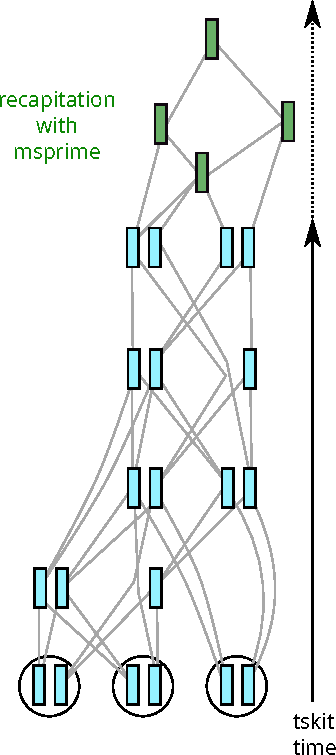
\includegraphics{figures/pedigree_recapitate}
    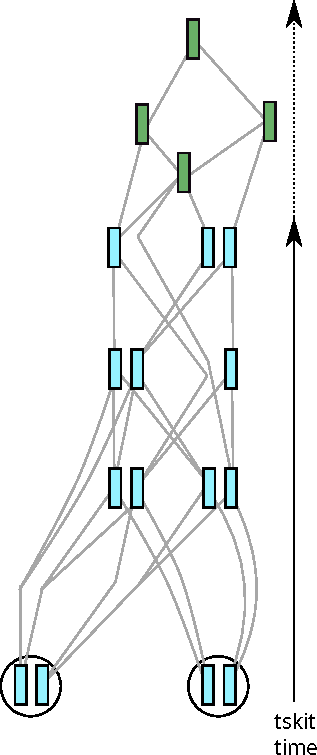
\includegraphics{figures/pedigree_simplify}
\caption{
    \textbf{(A)} Recapitation adds the green nodes by coalescent simulation.
    \textbf{(B)} Simplification.
}
\label{fig:recap_simp}
\end{figure}


Probably, your simulations have produced many more fictitious genomes
than you will be lucky enough to have in real life,
so at some point you may want to reduce your dataset to a realistic sample size.
We can get rid of unneeded samples and any extra information from them by using
an operation called *simplification* (this is the same basic approach that SLiM
implements under the hood when outputting a tree sequence).

Depicted in Figure~\ref{fig:recap_simp}B is the result of applying an explicit call to
simplify to our example tree sequence.
In the call we asked to keep only 4
genomes (contained in 2 of the individuals in the current generation). This has
substantially simplified the tree sequence, because only information relevant to the
genealogies of the 4 sample nodes has been kept. (Precisely, simplification retains only
nodes of the tree sequence that are branching points of some marginal genealogy -- see
CITE % [Kelleher et al 2018](https://doi.org/10.1371/journal.pcbi.1006581) for details.)
While simplification sounds very appealing - it makes things simpler after all -
it is often not necessary in practice, because tree sequences are very compact,
and many operations with them are quite fast.
(It will, however, speed up many operations, so if you plan to do a large number of simulations,
your workflow could benefit from early simplification.)
So, you should probably not make simplification a standard step in your workflow,
only using it if necessary.

It is important that simplification - if it happens at all -
either (a) comes after recapitation, or (b) is done with the
``keep\_input\_roots=True`` option.
This is because simplification removes some of the
ancestral genomes in the first generation,
which are necessary for recapitation,
unless it is asked to "keep the input roots".
If we simplify without this option before recapitating,
some of the first-generation blue chromosomes in the figure on the right
would not be present, so the coalescent simulation would start from a more recent point in time
than it really should.
As an extreme example, suppose our SLiM simulation has a single diploid who has reproduced
by clonal reproduction for 1,000 generations,
so that the final tree sequence is just two vertical lines of descent going back
to the two chromosomes in the initial individual alive 1,000 generations ago.
Recapitation would produce a shared history for these two chromosomes,
that would coalesce some time longer ago than 1,000 generations.
However, if we simplified first, then those two branches going back 1,000 generations would be removed,
since they don't convey any information about the shape of the tree;
and so recapitation might produce a common ancestor more recently than 1,000 generations,
which would be inconsistent with the SLiM simulation.

After recapitation,
simplification to the history of 100 individuals alive today
can be done with the {meth}`tskit.TreeSequence.simplify` method:
\begin{lstlisting}{language=slim}
import numpy as np
rng = np.random.default_rng(seed=3)
alive_inds = pyslim.individuals_alive_at(rts, 0)
keep_indivs = rng.choice(alive_inds, 100, replace=False)
keep_nodes = []
for i in keep_indivs:
  keep_nodes.extend(rts.individual(i).nodes)

sts = rts.simplify(keep_nodes, keep_input_roots=True)
\end{lstlisting}

Note that you must pass simplify a list of \textit{node IDs}, not individual IDs.
Here, we used the `.individuals\_alive\_at` method to obtain the list
of individuals alive today.
Also note that there are *still* more than 100 individuals remaining - 15 non-sample individuals
have not been simplified away,
because they have nodes that are required to describe the genealogies of the samples.
(Since this is a non-Wright-Fisher simulation,
parents and children can be both alive at the same time in the final generation.)



\subsection*{Adding neutral mutations to a SLiM simulation}

% ```{figure} _static/pedigree_mutate.png

If you have recorded a tree sequence in SLiM, likely you have not included any neutral mutations,
since it is much more efficient to simply add these on afterwards.
To add these (in a completely equivalent way to having included them during the simulation),
you can use the `msprime.sim\_mutations` function, which returns a new tree sequence with additional mutations.
Continuing with the cartoons from above, these are added to each branch of the tree sequence
at the rate per unit time that you request.
We'll add these using the {class}`msprime.SLiMMutationModel`, so that the file can be read back into SLiM,
but any of the other mutation models in msprime could be used.
This works as follows:
\begin{lstlisting}{language=slim}
next_id = pyslim.next_slim_mutation_id(sts)
ts = msprime.sim_mutations(
           sts,
           rate=1e-8,
           model=msprime.SLiMMutationModel(type=0, next_id=next_id),
           keep=True,
)
\end{lstlisting}


What's going on here? Let's step through the code.

\begin{enumerate}
    \item The mutation ``rate = 1e-8``, which adds mutations at a rate of $10^{-8}$ per bp.
    Unlike previous versions of msprime, this adds mutations using a discrete-sites model,
    i.e., only at integer locations (like SLiM).

\item We're passing ``type=0`` to the mutation model.
    This is because SLiM mutations need a "mutation type",
    and it makes the most sense if we add a type that was unused in the simulation.
    In this example we don't have any existing mutation types, so we can safely use ``type=0``.

\item We also add ``keep = True``, to keep any existing mutations.
    In this example there aren't any, so this isn't strictly necessary,
    but this is a good default.

\item If there are existing SLiM mutations on the tree sequence we need to
    make sure any newly added mutations have distinct SLiM IDs,
    so we use `.next\_slim\_mutation\_id` to figure out
    what the next available ID is, and pass it in.

\end{enumerate}

TODO: writing out to VCF


\section*{Parallelizing forward-in-time simulations of multiple species}

Any two branches stemming from the same node in a species tree are independent from each other and
thus can be simulated in parallel (assuming no migration between the species).
For example, in the phylogeny depicted in Figure~\ref{fig:phylo},
branches of the same color can be simulated in parallel.
To do so, we will need to
(i) simulate the history of each branch and
(ii) join the resulting simulations together onto one multi-species history.

 \begin{figure}[h!]
 \centering
  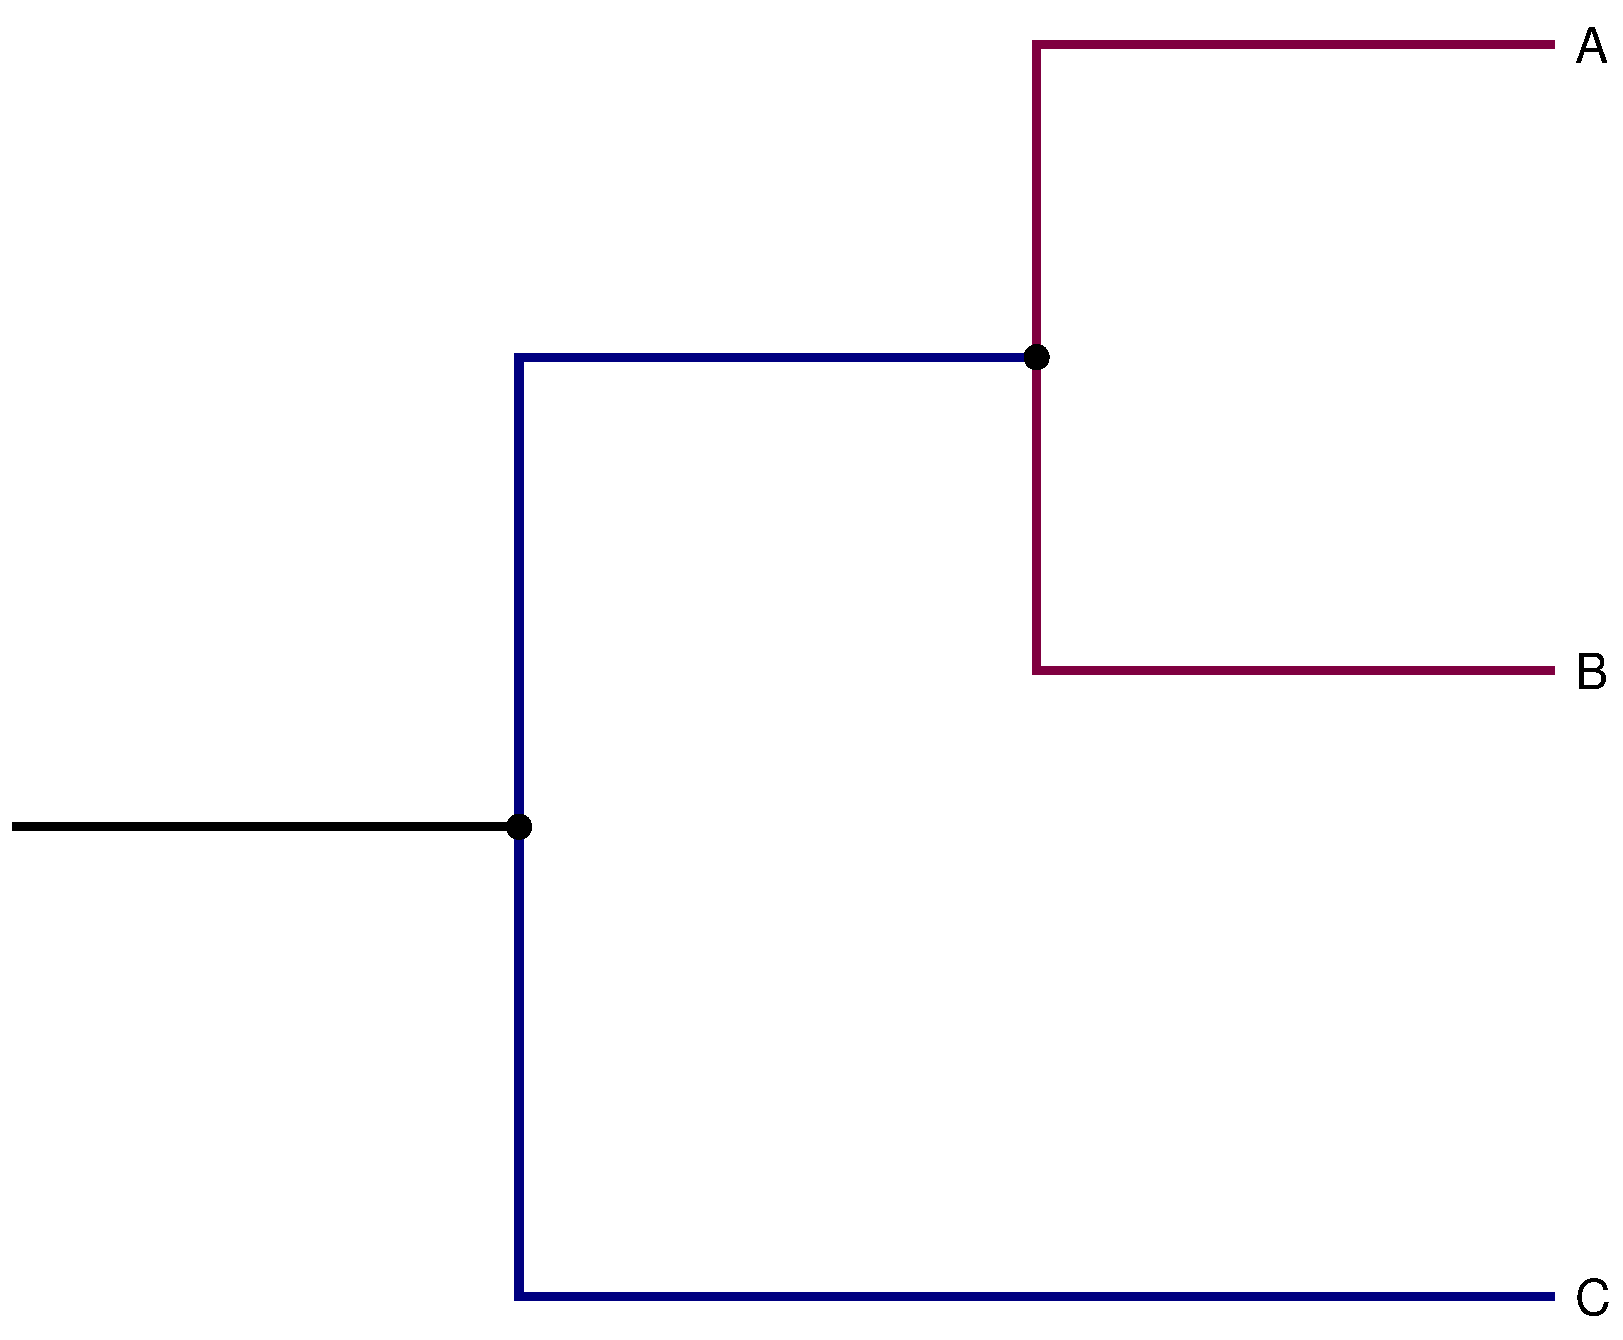
\includegraphics[width=0.5\textwidth]{./code/parallelizing_phylogeny/phylo.pdf}
  \caption{Example of phylogeny we might want to simulate. Note how branches with the same color can be simulated in parallel when there is no migration.}
  \label{fig:phylo}
 \end{figure}

\subsection{Parallel simulation of branches}

First, we need to write a \slim script that will be used for simulating the history of each branch in our phylogeny.
We will perform a simple simulation,
in which each branch can have a different (but fixed) population size and length (number of ticks).
Also, we will allow deleterious mutations to happen across the entire chromosome at a fixed rate.
See the code below (Listing~\ref{lst:slim-example}).

\begin{listing}[H]
  \inputminted[fontsize=\small, linenos, bgcolor=gray!10]{javascript}{./code/parallelizing_phylogeny/simulate_branch.slim}
  \caption{Simple \slim script to simulate a constant size population that can be started from an existing tree sequence.}
  \label{lst:slim-example}
\end{listing}

For each branch, the presence or absence of \verb|infile| tells \slim whether a previous branch exists or not.
If so, \slim will read the previous tree sequence and change the population size accordingly.
Note that when you read a tree sequence into \slim,
the tick counter will be updated with the time encoded in the tree sequence,
so we need to set the end of the simulation as the length of the branch (\verb|num_gens|)
plus the current “time” at the end of the loaded tree sequence.
At the end of the simulation, we call \verb|sim.treeSeqRememberIndividuals| right before saving the resulting tree sequence.
This is necessary because we need to ensure the individuals in the final generation are never dropped
from the tree sequence in future runs of \slim which are started from the output of the simulation,
as they will later be used to glue the tree sequences together.

The example phylogeny we will simulate is encoded in the table below (Table~\ref{tab:phylo}).

\begin{table}[H]
  \centering
  \caption{Parameters of the phylogeny that will be simulated.}
  \label{tab:phylo}
    \begin{tabular}{llll}
      \bfseries Child & \bfseries Parent & \bfseries Population size & \bfseries Edge length \\
      \hline
      \csvreader[head to column names]{./code/parallelizing_phylogeny/phylo.csv}{}%
        {\child & \parent & \popsize & \edgelen\\}
    \end{tabular}
\end{table}

\end{document}
